\chapter{La tabla de avance}\label{ch:g10:reaction-progress-table}

% ledger: use:NaN3-airbag
En un choque de coche, un cojín sale disparado del volante y se llena
de gas en una fracción de segundo, antes de que la cabeza del conductor
se desplace hacia delante. El gas lo produce una \omterm{def:g7:chemical-reactions:reaction}{reacción química}: una
pequeña carga de un sólido, la azida de sodio en el diseño clásico, se
descompone en sodio y nitrógeno. El ingeniero tiene que poner sólido
suficiente para llenar el cojín, pero no tanto que reviente, y no puede
quedar ningún \omterm{def:g7:chemical-reactions:reactant}{reactivo} que dañe a los pasajeros. ¿Cuánto sólido da
cuánto gas? Una \omterm{def:g8:balanced-equations:equation}{ecuación ajustada} da las proporciones; este capítulo las
convierte en una herramienta contable que sigue a cada \omterm{def:g7:chemical-reactions:reactant}{reactivo} y a cada
producto desde el principio de una reacción hasta el final.

\begin{recall}
Una \omterm{def:g8:balanced-equations:equation}{ecuación ajustada} mantiene igual en los dos miembros el número de
\omterm{def:g7:atoms-and-molecules:atom}{átomos} de cada elemento, y la carga; sus coeficientes dan las
proporciones en que reaccionan las especies (\cref{ch:g8:balanced-equations}).
La cantidad de una especie es $n = m/M$ para una masa, $n = V/V_m$ para
un gas (con $V_m = \qty{24.1}{L/mol}$ a \qty{20}{\celsius} y a la
presión atmosférica normal) (\cref{ch:g10:the-mole}), y $n = c \times V$
para un \omterm{def:g6:solutions-and-solubility:solute}{soluto}
(\cref{ch:g10:concentration-and-dilution}).
\end{recall}

\begin{omfigure}
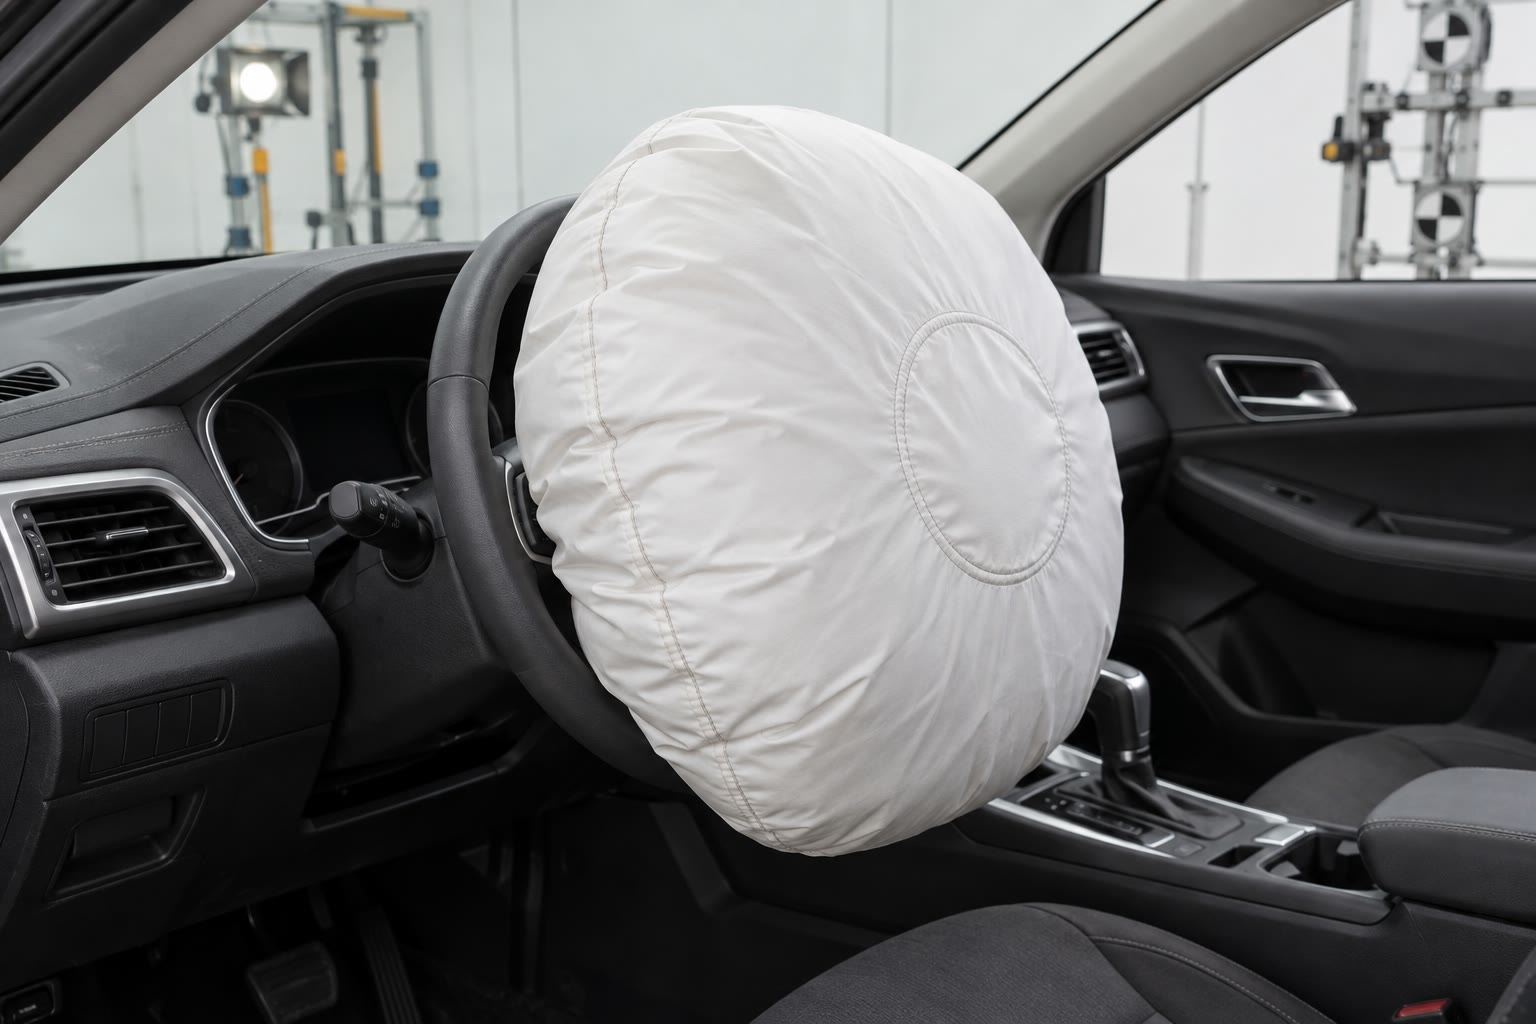
\includegraphics[width=0.5\linewidth]{images/book1/ai/g10-airbag.jpg}

{\small Un airbag se llena en una fracción de segundo con el nitrógeno
que produce una reacción.}
\end{omfigure}

\section{Describir un sistema químico}

\begin{definition}[Sistema químico, estados inicial y final]\label{def:g10:reaction-progress-table:system}
Un \emph{sistema químico}\index{sistema quimico@sistema químico} es el conjunto de
\omterm{def:g6:pure-substances-and-mixtures:species}{especies químicas} presentes en un lugar dado (un matraz, un cojín, una
pila), cada una con su cantidad y su estado físico. El sistema antes de
que empiece la reacción es el \emph{estado inicial}\index{estado inicial};
el sistema una vez que la reacción se ha detenido es el
\emph{estado final}\index{estado final}.
\end{definition}


\begin{example}[El metano arde en un recipiente cerrado]\label{ex:g10:reaction-progress-table:methane}
Un recipiente cerrado contiene \qty{2.0}{mol} de metano y \qty{3.0}{mol}
de dioxígeno; una chispa provoca la \omterm{def:g4:what-a-fire-needs:burning}{combustión}
\ce{CH4 + 2O2 -> CO2 + 2H2O}. En el \omterm{def:g10:reaction-progress-table:system}{estado inicial}, el sistema contiene
\qty{2.0}{mol} de \ce{CH4(g)}, \qty{3.0}{mol} de \ce{O2(g)} y ningún
producto. ¿Qué hay en el \omterm{def:g10:reaction-progress-table:system}{estado final}? El resto del capítulo lo
responde.
\end{example}

\section{El avance de la reacción y la tabla de avance}

\begin{definition}[Avance de la reacción, tabla de avance]\label{def:g10:reaction-progress-table:extent}
El \emph{avance de la reacción}\index{avance de la reaccion@avance de la reacción} $x$, en
\omterm{def:g10:the-mole:amount}{moles}, cuenta cuántas veces se ha producido la reacción tal como está
escrita en la \omterm{def:g8:balanced-equations:equation}{ecuación ajustada}: cuando el avance es $x$, una especie de
coeficiente $\nu$ se ha consumido (\omterm{def:g7:chemical-reactions:reactant}{reactivo}) o formado (producto) en la
cantidad $\nu x$. La \emph{tabla de avance}\index{tabla de avance} da,
debajo de la ecuación, la cantidad de cada especie en el \omterm{def:g10:reaction-progress-table:system}{estado
inicial}, para un avance $x$ y en el \omterm{def:g10:reaction-progress-table:system}{estado final}.
\end{definition}

\begin{method}[Rellenar una tabla de avance]\label{met:g10:reaction-progress-table:fill}
\begin{enumerate}
  \item Escribir la \omterm{def:g8:balanced-equations:equation}{ecuación ajustada} en la primera fila.
  \item \omterm{def:g10:reaction-progress-table:system}{Estado inicial} ($x = 0$): escribir debajo la cantidad inicial de
        cada especie.
  \item Estado intermedio (avance $x$): cada \omterm{def:g7:chemical-reactions:reactant}{reactivo} de coeficiente
        $\nu$ pasa a ser $n_0 - \nu x$, y cada producto, $n_0 + \nu x$.
  \item \omterm{def:g10:reaction-progress-table:system}{Estado final}: hallar $x_{\max}$ (sección siguiente) y llevarlo a
        las expresiones de la fila intermedia.
\end{enumerate}
\end{method}

\begin{omfigure}
\renewcommand{\arraystretch}{1.25}
\begin{tabular}{l|c|cccc}
\hline
ecuación & & \ce{CH4} & $+$ \ce{2O2} & $\longrightarrow$ \ce{CO2} & $+$ \ce{2H2O} \\
\hline
estado & avance (\si{mol}) & \multicolumn{4}{c}{cantidades (\si{mol})} \\
\hline
inicial & $0$ & $2.0$ & $3.0$ & $0$ & $0$ \\
intermedio & $x$ & $2.0 - x$ & $3.0 - 2x$ & $x$ & $2x$ \\
final & $x_{\max} = 1.5$ & $0.5$ & $0$ & $1.5$ & $3.0$ \\
\hline
\end{tabular}\par\medskip

{\small La \omterm{def:g10:reaction-progress-table:extent}{tabla de avance} de la \omterm{def:g4:what-a-fire-needs:burning}{combustión} del metano del ejemplo. Cada
columna sigue a una especie; los coeficientes 2 del \ce{O2} y del
\ce{H2O} se convierten en los $2x$.}
\end{omfigure}

\section{El reactivo limitante y el estado final}

\begin{definition}[Reactivo limitante, avance máximo, reacción total]\label{def:g10:reaction-progress-table:limiting}
Una reacción es una \emph{reacción total}\index{reaccion total@reacción total} si solo
se detiene cuando se agota uno de sus \omterm{def:g7:chemical-reactions:reactant}{reactivos}. Ese \omterm{def:g7:chemical-reactions:reactant}{reactivo} es el
\emph{reactivo limitante}\index{reactivo limitante}; los demás \omterm{def:g7:chemical-reactions:reactant}{reactivos}
están en exceso. El avance para el que se agota el \omterm{def:g7:chemical-reactions:reactant}{reactivo} limitante es
el \emph{avance máximo}\index{avance maximo@avance máximo} $x_{\max}$; el \omterm{def:g10:reaction-progress-table:system}{estado final}
de una reacción total es el estado en $x = x_{\max}$.
\end{definition}

\begin{method}[Hallar el reactivo limitante]\label{met:g10:reaction-progress-table:limiting}
\begin{enumerate}
  \item Para cada \omterm{def:g7:chemical-reactions:reactant}{reactivo}, resolver $n_0 - \nu x = 0$: el \omterm{def:g7:chemical-reactions:reactant}{reactivo} se
        agotaría en $x = n_0 / \nu$.
  \item El menor de estos valores es $x_{\max}$; el \omterm{def:g7:chemical-reactions:reactant}{reactivo} que lo da es
        el \omterm{def:g10:reaction-progress-table:limiting}{reactivo limitante}.
  \item Llevar $x_{\max}$ a la fila intermedia para obtener el \omterm{def:g10:reaction-progress-table:system}{estado
        final}; comprobar que ninguna cantidad es negativa.
\end{enumerate}
\end{method}

\begin{example}[Volvamos al metano]\label{ex:g10:reaction-progress-table:methane-final}
El metano se agotaría en $x = 2.0/1 = \qty{2.0}{mol}$, y el dioxígeno, en
$x = 3.0/2 = \qty{1.5}{mol}$. El menor es \qty{1.5}{mol}: el dioxígeno
es el \omterm{def:g10:reaction-progress-table:limiting}{reactivo limitante} y $x_{\max} = \qty{1.5}{mol}$. El \omterm{def:g10:reaction-progress-table:system}{estado final}
contiene \qty{0.5}{mol} de metano sobrante, nada de dioxígeno,
\qty{1.5}{mol} de dióxido de carbono y \qty{3.0}{mol} de agua.
\end{example}

\begin{omfigure}
\begin{tikzpicture}
\begin{axis}[width=0.78\linewidth, height=6.2cm, xmin=0, xmax=2.05,
    ymin=0, ymax=4.2, xlabel={avance $x$ (\si{mol})},
    ylabel={cantidad (\si{mol})}, axis lines*=left, ymajorgrids,
    grid style={gray!20}, tick label style={font=\small},
    label style={font=\small}, xtick={0,0.5,1,1.5,2},
    legend style={font=\small, at={(1.02,0.5)}, anchor=west, draw=none},
    legend cell align=left]
  \addplot[very thick, omDef, domain=0:2] {2-x};
  \addplot[very thick, omThm, domain=0:1.5] {3-2*x};
  \addplot[very thick, omMeth, domain=0:2] {x};
  \addplot[very thick, omProp, domain=0:2] {2*x};
  \legend{\ce{CH4}, \ce{O2}, \ce{CO2}, \ce{H2O}}
  \addplot[dashed, black!60] coordinates {(1.5,0) (1.5,4.2)};
  \node[font=\small, anchor=south west] at (axis cs:1.5,3.55) {$x_{\max}$};
  \fill[black!8, opacity=0.6] (axis cs:1.5,0) rectangle (axis cs:2.05,4.2);
\end{axis}
\end{tikzpicture}

{\small Las cantidades en función del avance para el ejemplo del metano.
El dioxígeno (rojo) llega primero a cero, en $x = \qty{1.5}{mol}$: la
reacción se detiene ahí, y la parte sombreada no se alcanza nunca.}
\end{omfigure}

\begin{remark}[No todas las reacciones son totales]\label{rem:g10:reaction-progress-table:not-total}
Muchas reacciones se detienen antes de que se agote ningún \omterm{def:g7:chemical-reactions:reactant}{reactivo}:
llegan a un estado en el que coexisten \omterm{def:g7:chemical-reactions:reactant}{reactivos} y productos. Su \omterm{def:g10:reaction-progress-table:system}{estado
final} no es $x_{\max}$, y un capítulo posterior enseña a hallarlo. En
este capítulo, todas las reacciones son totales.
\end{remark}

\section{La mezcla estequiométrica}

\begin{definition}[Mezcla estequiométrica]\label{def:g10:reaction-progress-table:stoichiometric}
Una \omterm{def:g6:pure-substances-and-mixtures:mixture}{mezcla} de \omterm{def:g7:chemical-reactions:reactant}{reactivos} es una \emph{mezcla
estequiométrica}\index{mezcla estequiometrica@mezcla estequiométrica} cuando las cantidades
iniciales están en las proporciones de los coeficientes de la \omterm{def:g8:balanced-equations:equation}{ecuación
ajustada}.
\end{definition}

\begin{proposition}[Todos los reactivos se agotan a la vez]\label{prop:g10:reaction-progress-table:together}
Para una reacción $a\,\ce{A} + b\,\ce{B} \longrightarrow$ productos, la \omterm{def:g6:pure-substances-and-mixtures:mixture}{mezcla} es estequiométrica si
y solo si
\[
  \frac{n_0(\ce{A})}{a} = \frac{n_0(\ce{B})}{b},
\]
y entonces, en una \omterm{def:g10:reaction-progress-table:limiting}{reacción total}, los dos \omterm{def:g7:chemical-reactions:reactant}{reactivos} se consumen por
completo en el \omterm{def:g10:reaction-progress-table:system}{estado final}.
\end{proposition}

\begin{proof}
\ce{A} se agotaría en $x = n_0(\ce{A})/a$, y \ce{B}, en $x = n_0(\ce{B})/b$.
Los dos valores son iguales exactamente cuando las proporciones son las
de la ecuación, y entonces el avance $x_{\max}$ los agota a los dos a la
vez.
\end{proof}

\begin{example}[Quemar metano limpiamente]\label{ex:g10:reaction-progress-table:stoich}
Para \ce{CH4 + 2O2 -> CO2 + 2H2O}, \qty{2.0}{mol} de metano necesitan
\qty{4.0}{mol} de dioxígeno: $2.0/1 = 4.0/2$. Con solo \qty{3.0}{mol} de
dioxígeno, a la \omterm{def:g6:pure-substances-and-mixtures:mixture}{mezcla} del primer ejemplo le faltaba oxígeno; en una
llama real, esa falta es lo que produce el venenoso monóxido de carbono
(\cref{ch:g8:combustion-and-fuels}).
\end{example}

\section{Gases y disoluciones en la tabla}


\begin{method}[Cantidades del estado inicial]\label{met:g10:reaction-progress-table:amounts}
Antes de rellenar una tabla, se convierte en cantidad cada magnitud
dada: $n = m/M$ para un sólido o un líquido pesado; $n = V/V_m$ para un
gas; $n = c \times V$ para una especie disuelta. Al final, las
cantidades del \omterm{def:g10:reaction-progress-table:system}{estado final} se vuelven a convertir en lo que se pida:
masa, volumen de gas o concentración.
\end{method}

\begin{example}[El magnesio en ácido clorhídrico]\label{ex:g10:reaction-progress-table:magnesium}
% ledger: aw:Mg
El ácido clorhídrico contiene \omterm{def:g9:ions:ion}{iones} hidrógeno \ce{H+}, que atacan el
magnesio: \ce{Mg + 2H+ -> Mg^{2+} + H2}. Se echa una cinta de
\qty{0.12}{g} de magnesio en \qty{50.0}{mL} de ácido con
$c(\ce{H+}) = \qty{1.0}{mol/L}$. Cantidades iniciales:
$n_0(\ce{Mg}) = 0.12/24.3 = \qty{4.9e-3}{mol}$ y
$n_0(\ce{H+}) = 1.0 \times 0.0500 = \qty{5.0e-2}{mol}$. El magnesio se
agotaría en $x = \qty{4.9e-3}{mol}$, y los \omterm{def:g9:ions:ion}{iones} hidrógeno, en
$x = 0.050/2 = \qty{2.5e-2}{mol}$: el magnesio es el limitante y
$x_{\max} = \qty{4.9e-3}{mol}$. La reacción da \qty{4.9e-3}{mol} de
dihidrógeno, es decir, $\num{4.9e-3} \times 24.1 = \qty{0.12}{L}$ a
\qty{20}{\celsius}, y deja $0.050 - 2 \times 0.0049 =
\qty{0.040}{mol}$ de \omterm{def:g9:ions:ion}{iones} hidrógeno en exceso.
\end{example}

\begin{inthelab}[Globos sobre matraces]
El profesor vierte \qty{50.0}{mL} del mismo ácido clorhídrico en cada
uno de seis matraces Erlenmeyer, y pone en seis globos masas crecientes
de magnesio en polvo: 0.15, 0.30, 0.45, 0.60, 0.75 y \qty{0.90}{g}.
Ajusta cada globo a la boca de su matraz y luego lo levanta para que el
polvo caiga en el ácido. Los globos se hinchan mientras la \omterm{def:g6:pure-substances-and-mixtures:mixture}{mezcla}
burbujea. Cuando todo se ha detenido, los globos son cada vez más
grandes del primer matraz al cuarto; el cuarto, el quinto y el sexto
tienen el mismo tamaño, y en los dos últimos queda algo de polvo gris en
el fondo del matraz.
\end{inthelab}

\begin{omfigure}
\begin{tikzpicture}[font=\small, scale=0.82]
  % H2 volume (L): 0.149 0.298 0.446 0.595 0.6025 0.6025; radius ~ V^(1/3)
  \foreach \i/\m/\v/\r/\left in {0/0.15/0.15/0.42/0, 1/0.30/0.30/0.53/0,
      2/0.45/0.45/0.61/0, 3/0.60/0.60/0.67/0, 4/0.75/0.60/0.67/1,
      5/0.90/0.60/0.67/1} {
    \begin{scope}[shift={(2.35*\i,0)}]
      \pic[transform shape] at (0,0) {erlenmeyer={0.25}{omWater}};
      \ifnum\left=1
        \fill[black!45] (-0.5,0.03) rectangle (0.5,0.12);
      \fi
      \fill[omProp!35, draw=omProp!80!black] (-0.3,2.6) -- (0.3,2.6)
        -- (0.12,2.82) -- (-0.12,2.82) -- cycle;
      \shade[ball color=omProp!40, draw=omProp!80!black]
        (0,{2.78+\r}) circle (\r);
      \node[align=center, anchor=north] at (0,-0.15)
        {\qty{\m}{g} Mg\\ \qty{\v}{L}};
    \end{scope}
  }
\end{tikzpicture}

{\small Seis matraces con el mismo ácido y masas crecientes de magnesio,
con el volumen de dihidrógeno (a \qty{20}{\celsius}) de cada globo. A
partir de unos \qty{0.61}{g}, el limitante es el ácido: los globos dejan
de crecer y sobra magnesio (gris).}
\end{omfigure}

\begin{remark}[Leer la meseta]\label{rem:g10:reaction-progress-table:plateau}
En los primeros matraces, el magnesio es el \omterm{def:g10:reaction-progress-table:limiting}{reactivo limitante}, y
duplicarlo duplica el gas. A partir de cierta masa, los \omterm{def:g9:ions:ion}{iones} hidrógeno
se agotan primero: añadir magnesio no cambia nada salvo el polvo que
sobra. El cambio se produce exactamente en la \omterm{def:g10:reaction-progress-table:stoichiometric}{mezcla estequiométrica},
$n_0(\ce{Mg}) = n_0(\ce{H+})/2 = \qty{0.025}{mol}$, es decir,
$0.025 \times 24.3 = \qty{0.61}{g}$ de magnesio.
\end{remark}

\begin{safety}{\ghs[0.82cm]{GHS02}\ghs[0.82cm]{GHS05}\ghs[0.82cm]{GHS07}}
% ledger: ghs:Mg, ghs:HCl
El magnesio en polvo es inflamable; el ácido clorhídrico quema la piel y
los ojos y sus vapores irritan las vías respiratorias; el dihidrógeno
\omterm{def:g4:what-a-fire-needs:burning}{arde} en el \omterm{def:g4:air-a-mixture-of-gases:air}{aire}. Una demostración que hace el profesor, con gafas, lejos
de cualquier llama.
\end{safety}

\section{Ejercicios}

\begin{exercise}[$\star$]\label{exo:g10:reaction-progress-table:1}
Rellena la \omterm{def:g10:reaction-progress-table:extent}{tabla de avance} de \ce{2H2 + O2 -> 2H2O} para una \omterm{def:g6:pure-substances-and-mixtures:mixture}{mezcla}
inicial de \qty{4.0}{mol} de dihidrógeno y \qty{3.0}{mol} de dioxígeno,
suponiendo que la reacción es total. Da $x_{\max}$, el \omterm{def:g10:reaction-progress-table:limiting}{reactivo
limitante} y el \omterm{def:g10:reaction-progress-table:system}{estado final}.
\end{exercise}

\begin{exercise}[$\star$]\label{exo:g10:reaction-progress-table:2}
El carbono \omterm{def:g4:what-a-fire-needs:burning}{arde} en dioxígeno: \ce{C + O2 -> CO2}. A partir de
\qty{3.0}{mol} de carbono y \qty{2.0}{mol} de dioxígeno, halla
$x_{\max}$, el \omterm{def:g10:reaction-progress-table:limiting}{reactivo limitante} y el \omterm{def:g10:reaction-progress-table:system}{estado final}.
\end{exercise}

\begin{exercise}[$\star$]\label{exo:g10:reaction-progress-table:3}
El hierro y el azufre reaccionan al calentarlos: \ce{Fe + S -> FeS}. A
partir de \qty{0.50}{mol} de hierro y \qty{0.30}{mol} de azufre,
describe el \omterm{def:g10:reaction-progress-table:system}{estado final}.
\end{exercise}

\begin{exercise}[$\star$]\label{exo:g10:reaction-progress-table:4}
Supón que la reacción \ce{N2 + 3H2 -> 2NH3} es total. A partir de
\qty{1.0}{mol} de dinitrógeno y \qty{2.4}{mol} de dihidrógeno, halla
$x_{\max}$ y el \omterm{def:g10:reaction-progress-table:system}{estado final}.
\end{exercise}

\begin{exercise}[$\star$]\label{exo:g10:reaction-progress-table:5}
Para \ce{2CO + O2 -> 2CO2}, ¿cuál de estas \omterm{def:g6:pure-substances-and-mixtures:mixture}{mezclas} es estequiométrica?
(a) \qty{2}{mol} de \ce{CO} y \qty{2}{mol} de \ce{O2}; (b) \qty{4}{mol}
de \ce{CO} y \qty{2}{mol} de \ce{O2}; (c) \qty{1}{mol} de \ce{CO} y
\qty{2}{mol} de \ce{O2}.
\end{exercise}

\begin{exercise}[$\star\star$]\label{exo:g10:reaction-progress-table:6}
¿Qué masa de dioxígeno hace falta para quemar por completo \qty{32}{g}
de metano (\ce{CH4 + 2O2 -> CO2 + 2H2O})? ¿Qué masa de agua se forma?
\end{exercise}

\begin{exercise}[$\star\star$]\label{exo:g10:reaction-progress-table:7}
Un hornillo de camping quema \qty{1.0}{kg} de propano:
\ce{C3H8 + 5O2 -> 3CO2 + 4H2O}. ¿Qué volumen de dióxido de carbono, a
\qty{20}{\celsius}, libera?
\end{exercise}

\begin{exercise}[$\star\star$]\label{exo:g10:reaction-progress-table:8}
Con la figura de las cantidades en función del avance del ejemplo del
metano, lee las cantidades de las cuatro especies en
$x = \qty{1.0}{mol}$. ¿Por qué la línea del dioxígeno se detiene en
$x = \qty{1.5}{mol}$?
\end{exercise}

\begin{exercise}[$\star\star$]\label{exo:g10:reaction-progress-table:9}
Se añaden \qty{1.30}{g} de cinc en polvo a \qty{100.0}{mL} de
disolución azul de sulfato de cobre de \qty{0.10}{mol/L}. La reacción es
\ce{Zn + Cu^{2+} -> Zn^{2+} + Cu}.
Halla el \omterm{def:g10:reaction-progress-table:limiting}{reactivo limitante}, la masa de cobre formada y la masa de cinc
que queda. ¿Sigue azul la disolución al final?
\end{exercise}

\begin{exercise}[$\star\star$]\label{exo:g10:reaction-progress-table:10}
Se añaden \qty{0.48}{g} de magnesio a \qty{20.0}{mL} de ácido
clorhídrico con $c(\ce{H+}) = \qty{1.0}{mol/L}$
(\ce{Mg + 2H+ -> Mg^{2+} + H2}). ¿Qué \omterm{def:g7:chemical-reactions:reactant}{reactivo} es el limitante? ¿Qué
volumen de dihidrógeno se recoge a \qty{20}{\celsius}?
\end{exercise}

\begin{exercise}[$\star\star$]\label{exo:g10:reaction-progress-table:11}
En el ejercicio~3, ¿en qué porcentaje supera el \omterm{def:g7:chemical-reactions:reactant}{reactivo} en exceso la
cantidad que habría dado una \omterm{def:g10:reaction-progress-table:stoichiometric}{mezcla estequiométrica}?
\end{exercise}

\begin{exercise}[$\star\star\star$]\label{exo:g10:reaction-progress-table:12}
Un alumno quiere \qty{10.0}{g} de una \omterm{def:g10:reaction-progress-table:stoichiometric}{mezcla estequiométrica} de hierro y
azufre para \ce{Fe + S -> FeS}. ¿Qué masas de hierro y de azufre debe
pesar?
\end{exercise}

\begin{exercise}[$\star\star\star$]\label{exo:g10:reaction-progress-table:13}
Se calientan fuertemente \qty{10.0}{g} de caliza \ce{CaCO3}, que se
descompone totalmente: \ce{CaCO3 -> CaO + CO2}. La cal viva \ce{CaO}
obtenida se pone después en \qty{1.8}{g} de agua:
\ce{CaO + H2O -> Ca(OH)2}.
\begin{enumerate}
  \item Rellena la \omterm{def:g10:reaction-progress-table:extent}{tabla de avance} de la primera reacción; ¿qué volumen
        de dióxido de carbono se libera a \qty{20}{\celsius}?
  \item Rellena la tabla de la segunda reacción. ¿Qué \omterm{def:g7:chemical-reactions:reactant}{reactivo} es el
        limitante? ¿Qué masa de cal apagada \ce{Ca(OH)2} se forma?
\end{enumerate}
\end{exercise}

\begin{exercise}[$\star\star\star$]\label{exo:g10:reaction-progress-table:14}
En el experimento de los globos del recuadro de laboratorio, calcula el
volumen de dihidrógeno de cada globo. Explica por qué deja de crecer
después del cuarto matraz, y representa (a mano) el volumen de gas en
función de la masa de magnesio.
\end{exercise}

\begin{exercise}[$\star\star\star$]\label{exo:g10:reaction-progress-table:15}
Se queman \qty{4.6}{g} de etanol \ce{C2H6O} en un recipiente cerrado
que contiene \qty{4.8}{L} de dioxígeno a \qty{20}{\celsius}:
\ce{C2H6O + 3O2 -> 2CO2 + 3H2O}. Halla el \omterm{def:g10:reaction-progress-table:limiting}{reactivo limitante}, la masa
de etanol que queda sin quemar y el volumen de dióxido de carbono
formado.
\end{exercise}

\section{Problema: El airbag}

\begin{problem}[{Problema de fin de semana --- ¿qué masa de azida de
sodio hay que meter en un volante para llenar un airbag de 60 litros?}]
\label{pb:g10:reaction-progress-table:1}
% ledger: use:NaN3-airbag, ghs:NaN3, aw:Na, aw:N, aw:K, aw:O
En el diseño clásico de un airbag, una chispa eléctrica provoca la
descomposición de la azida de sodio sólida:
\[
  \ce{2NaN3 -> 2Na + 3N2} .
\]
El sodio metálico que se forma es peligroso: reacciona violentamente
con el agua, y con la humedad de la piel y de los ojos. Por eso la carga
contiene también nitrato de potasio, que convierte el sodio en óxidos
inofensivos y da un poco más de nitrógeno:
\[
  \ce{10Na + 2KNO3 -> K2O + 5Na2O + N2} .
\]
Las dos reacciones son totales. El airbag tiene que llenarse con
\qty{60}{L} de nitrógeno; toma el gas a \qty{20}{\celsius}, donde
$V_m = \qty{24.1}{L/mol}$.

\medskip
\noindent\textbf{Parte I --- Las reacciones.}
\begin{enumerate}
  \item Comprueba que la primera ecuación está ajustada, elemento por
        elemento.
  \item Comprueba que la segunda ecuación está ajustada.
  \item ¿Qué capítulo anterior mostró que el sodio reacciona
        violentamente con el agua? ¿Por qué no debe quedar nada de sodio
        después del choque?
  \item Calcula las \omterm{def:g10:the-mole:molar-mass}{masas molares} de la azida de sodio \ce{NaN3} y del
        nitrato de potasio \ce{KNO3}.
\end{enumerate}

\medskip
\noindent\textbf{Parte II --- La descomposición.}
\begin{enumerate}[resume]
  \item Rellena la \omterm{def:g10:reaction-progress-table:extent}{tabla de avance} de la primera reacción para una
        cantidad inicial de \qty{1.00}{mol} de azida de sodio.
  \item Halla $x_{\max}$. ¿Cuál es el \omterm{def:g10:reaction-progress-table:limiting}{reactivo limitante}?
  \item Da las cantidades de sodio y de nitrógeno del \omterm{def:g10:reaction-progress-table:system}{estado final}.
  \item ¿Qué volumen de nitrógeno da \qty{1.00}{mol} de azida de sodio a
        \qty{20}{\celsius}?
\end{enumerate}

\medskip
\noindent\textbf{Parte III --- Eliminar el sodio.}
\begin{enumerate}[resume]
  \item Rellena la \omterm{def:g10:reaction-progress-table:extent}{tabla de avance} de la segunda reacción, a partir del
        sodio hallado en la pregunta 7 y de una cantidad $n$ de nitrato
        de potasio.
  \item ¿Qué cantidad, y qué masa, de nitrato de potasio forma una
        \omterm{def:g10:reaction-progress-table:stoichiometric}{mezcla estequiométrica} con este sodio?
  \item Da el \omterm{def:g10:reaction-progress-table:system}{estado final} de la segunda reacción para esta \omterm{def:g6:pure-substances-and-mixtures:mixture}{mezcla}.
  \item Si solo se pusieran \qty{0.150}{mol} de nitrato de potasio, ¿qué
        \omterm{def:g7:chemical-reactions:reactant}{reactivo} sería el limitante, y qué quedaría? ¿Por qué sería
        peligroso?
\end{enumerate}

\medskip
\noindent\textbf{Parte IV --- El airbag de 60 litros.}
\begin{enumerate}[resume]
  \item A partir de las preguntas 7 y 11, ¿qué cantidad de nitrógeno da
        la carga completa por cada \omterm{def:g10:the-mole:amount}{mol} de azida de sodio?
  \item ¿Qué cantidad de nitrógeno llena el airbag?
  \item Deduce la cantidad de azida de sodio necesaria.
  \item Calcula su masa.
  \item Calcula la masa de nitrato de potasio que hay que añadir.
  \item Sin la segunda reacción, ¿qué masa de azida de sodio habría
        hecho falta? ¿Cuánto ahorra la segunda reacción?
  \item La azida de sodio es mortal en caso de ingestión. ¿Por qué
        importa que la primera reacción sea total, y cómo muestra la
        \omterm{def:g10:reaction-progress-table:extent}{tabla de avance} que no queda nada?
  \item Da la respuesta final: ¿qué masa de azida de sodio llena un
        airbag de \qty{60}{L}?
\end{enumerate}
\end{problem}
